\documentclass[11pt, letterpaper]{article}

\usepackage[margin=1in]{geometry}
\usepackage{amsmath, amssymb}
\usepackage{mathpazo} % Palatino font for a nice look
\usepackage{enumitem}
\usepackage{titlesec}
\usepackage{fancyhdr}
\usepackage{xcolor}
\usepackage{mdframed}
\usepackage{tikz}

% Setup header/footer
\pagestyle{fancy}
\fancyhf{}
\rhead{Health Economics -- Assignment 3}
\lhead{Name: Xuange Liang (xl3493)}
\cfoot{Page \thepage}
\renewcommand{\headrulewidth}{0.4pt}

% Format section titles
\titleformat{\section}{\large\bfseries\color{blue!60!black}}{}{0em}{}[\vspace{-0.5em}\rule{\textwidth}{0.5pt}]

\setlength{\parindent}{0pt}
\setlength{\parskip}{0.8em}

\begin{document}

\begin{center}
    \LARGE\bfseries Health Economics -- Assignment 3
\end{center}
\vspace{1em}

\section*{1. Consider a perfectly competitive market for generic insulin. Draw a graph showing both the market equilibrium and an individual firm's demand curve in a perfectly competitive market. Label the market equilibrium price (P*) and quantity (Q*), and explain why the individual firm faces a horizontal demand curve even though the market demand curve is downward sloping. (4 points)}

\begin{center}
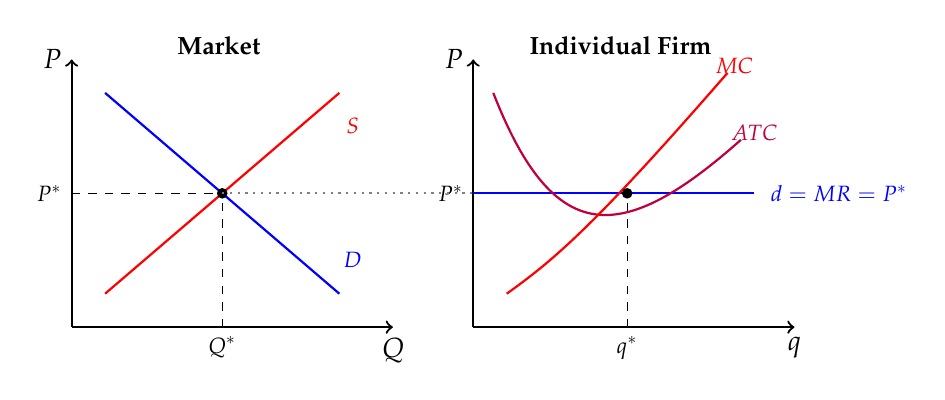
\begin{tikzpicture}[scale=0.85]
    % Market Graph
    \node[font=\small\bfseries] at (2.2, 4.2) {Market};
    \draw[->, thick] (0,0) -- (4.8,0) node[below] {$Q$};
    \draw[->, thick] (0,0) -- (0,4) node[left] {$P$};
    \draw[thick, blue] (0.5,3.5) -- (4,0.5);
    \node[blue, font=\footnotesize] at (4.2,1) {$D$};
    \draw[thick, red] (0.5,0.5) -- (4,3.5);
    \node[red, font=\footnotesize] at (4.2,3) {$S$};
    \draw[dashed] (2.25,0) node[below] {\footnotesize $Q^*$} -- (2.25,2);
    \draw[dashed] (0,2) node[left] {\footnotesize $P^*$} -- (2.25,2);
    \filldraw[black] (2.25,2) circle (2pt);
    
    % Firm Graph
    \begin{scope}[shift={(6,0)}]
        \node[font=\small\bfseries] at (2.2, 4.2) {Individual Firm};
        \draw[->, thick] (0,0) -- (4.8,0) node[below] {$q$};
        \draw[->, thick] (0,0) -- (0,4) node[left] {$P$};
        % d = MR = P* (horizontal demand)
        \draw[thick, blue] (0,2) -- (4.2,2);
        \node[blue, font=\footnotesize, anchor=west] at (4.3,2) {$d = MR = P^*$};
        \node[left, font=\footnotesize] at (0,2) {$P^*$};
        % ATC curve (U-shaped, minimum near q*)
        \draw[thick, purple] (0.3,3.5) .. controls (1.2,1.2) and (2.2,1.2) .. (4.0,2.8);
        \node[purple, font=\footnotesize] at (4.2,2.9) {$ATC$};
        % MC curve (upward sloping, crosses ATC at its minimum)
        \draw[thick, red] (0.5,0.5) .. controls (1.2,1.0) and (1.8,1.5) .. (3.8,3.8);
        \node[red, font=\footnotesize] at (3.9,3.9) {$MC$};
        % q* at MR=MC intersection (~q=2.3)
        \draw[dashed] (2.3,0) node[below] {\footnotesize $q^*$} -- (2.3,2);
        \filldraw[black] (2.3,2) circle (2pt);
    \end{scope}
    
    % Connecting arrow
    \draw[dotted, thick, gray] (2.25,2) -- (6,2);
\end{tikzpicture}
\end{center}

\textbf{Explanation}: 
In a perfectly competitive market, there are many producers selling identical (homogeneous) products, such as generic insulin. Because each individual firm is very small relative to the entire market, it has no market power to influence the market price. If a firm tries to charge even slightly more than the prevailing market price ($P^*$), consumers will simply buy from countless other competitors, dropping the firm's sales to zero. As a result, the firm is a \textit{price taker} and faces a perfectly elastic (horizontal) demand curve at $P^*$, meaning it can sell any quantity it wishes exactly at the market price, regardless of the downward-sloping nature of the overall market demand.

\section*{2. Define market power. Discuss price takers and price setters and give examples. (2 points)}

\textbf{Market Power} is the ability of a firm to raise and maintain the price of its product or service above the level that would prevail under perfectly competitive conditions, without losing all of its customers.

\begin{itemize}[leftmargin=*]
    \item \textbf{Price Takers}: Firms with absolutely zero market power. Because they face intense competition and sell interchangeable goods, they must accept the prevailing market price as given. \textit{Example}: A small wheat farmer or a manufacturer of standard generic ibuprofen.
    \item \textbf{Price Setters}: Firms possessing market power. Because they offer unique or differentiated products with significant barriers to entry, they face a downward-sloping demand curve and can actively choose their profit-maximizing price. \textit{Example}: A pharmaceutical company holding an exclusive patent for a breakthrough biologic drug.
\end{itemize}

\section*{3. Define deadweight loss and list two causes of market failure that can lead to deadweight loss. For each cause, provide an example. (2 points)}

\textbf{Deadweight Loss (DWL)} is the net loss of total economic surplus (the sum of consumer and producer surplus) that occurs when an inefficient outcome is reached and the market fails to produce the socially optimal quantity of a good or service.

\textbf{Causes of Market Failure resulting in DWL}:
\begin{enumerate}[leftmargin=*]
    \item \textbf{Externalities}: Occurs when a transaction imposes uncompensated costs or benefits on third parties not involved in the trade. \\
    \textit{Example}: A pharmaceutical plant polluting a local river during production (negative production externality), creating health hazards for nearby residents and leading to overproduction relative to the socially efficient level.
    \item \textbf{Market Power (Monopoly)}: Occurs when a single seller controls the market and restricts output below the competitive level to artificially inflate prices and maximize profit. \\
    \textit{Example}: A monopolist holding a life-saving drug patent artificially restricting the drug's supply to charge a high premium, pricing out patients who value the drug above its marginal cost of production.
\end{enumerate}

\section*{4. Consider the market for prescription opioids. Assume that opioid misuse creates negative externalities through increased addiction, overdose deaths, and healthcare costs borne by society.}

\textbf{a) Draw a graph showing the market for prescription opioids with a negative consumption externality. Your graph should include: MPB, MSB, MPC=MSC, Market equilibrium ($Q_0$), socially efficient quantity ($Q_1$). (4 points)}
\begin{center}
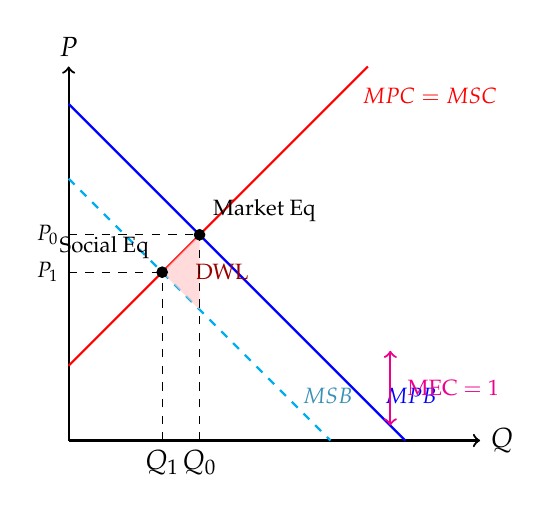
\begin{tikzpicture}[scale=0.95]
    % Axes
    \draw[->, thick] (0,0) -- (5.5,0) node[right] {$Q$};
    \draw[->, thick] (0,0) -- (0,5) node[above] {$P$};
    
    % MPB: P = 5 - Q (intersects at Q=5, P=0 and Q=0, P=5)
    \draw[thick, blue] (0,4.5) -- (4.5,0);
    \node[blue, font=\footnotesize, anchor=west] at (4.1,0.6) {$MPB$};
    
    % MSB: P = 4 - Q  (shifted down by MEC=1)
    \draw[thick, cyan, dashed] (0,3.5) -- (3.5,0);
    \node[cyan!70!black, font=\footnotesize, anchor=west] at (3.0,0.6) {$MSB$};
    
    % MPC=MSC: P = 1 + Q
    \draw[thick, red] (0,1) -- (4,5);
    \node[red, font=\footnotesize, anchor=west] at (3.8,4.6) {$MPC=MSC$};
    
    % Curves: MPB: P=4.5-Q, MSB: P=3.5-Q (MEC=1), MSC: P=1+Q
    % Market Eq (MPB=MSC): 4.5-Q=1+Q => Q0=1.75, P0=2.75
    % Social Eq (MSB=MSC): 3.5-Q=1+Q => Q1=1.25, P1=2.25
    % DWL triangle vertices: Social Eq (1.25,2.25), MSB@Q0=(1.75,1.75), Market Eq (1.75,2.75)
    \fill[red!20, opacity=0.7] (1.25,2.25) -- (1.75,1.75) -- (1.75,2.75) -- cycle;
    \node[red!60!black, font=\footnotesize] at (2.05, 2.25) {DWL};

    % Market Eq
    \draw[dashed] (1.75,0) node[below] {$Q_0$} -- (1.75,2.75);
    \draw[dashed] (0,2.75) node[left] {\footnotesize $P_0$} -- (1.75,2.75);
    \filldraw[black] (1.75,2.75) circle (2pt);
    \node[font=\footnotesize, anchor=south west] at (1.8,2.8) {Market Eq};

    % Social Eq
    \draw[dashed] (1.25,0) node[below] {$Q_1$} -- (1.25,2.25);
    \draw[dashed] (0,2.25) node[left] {\footnotesize $P_1$} -- (1.25,2.25);
    \filldraw[black] (1.25,2.25) circle (2pt);
    \node[font=\footnotesize, anchor=south east] at (1.2,2.3) {Social Eq};

    % MEC annotation (vertical bracket showing gap between MPB and MSB)
    \draw[<->, thick, magenta] (4.3, 0.2) -- (4.3, 1.2);
    \node[magenta, font=\footnotesize, anchor=west] at (4.4, 0.7) {MEC $= 1$};
\end{tikzpicture}
\end{center}

\textbf{b) Does the unregulated market produce too much or too little relative to the socially efficient quantity? Explain why in 2-3 sentences. (2 points)} \\
The unregulated market produces \textbf{too much} relative to the socially efficient quantity ($Q_0 > Q_1$). This happens because consumers and producers only consider their own Private Marginal Benefits and Private Marginal Costs when transacting, completely ignoring the external damages (addiction, healthcare burdens) they impose on society. Consequently, the drug is over-consumed beyond the point where the marginal social cost outweighs the marginal social benefit.

\textbf{c) Propose one government intervention that could move the market toward the socially efficient outcome and explain how it would work. (2 points)} \\
The government could impose a \textbf{Pigouvian Tax} on prescription opioids exactly equal to the Marginal External Cost (MEC) evaluated at the socially optimal output level. This tax would shift the private supply curve ($MPC$) upwards so that consumers and producers "internalize the externality", effectively raising the market price and reducing the equilibrium purchase quantity down to the socially efficient level ($Q_1$).

\section*{5. A biotechnology company... Demand: $P = 200 - 5Q$, Total Cost: $TC = 500 + 10Q + 20Q^2$, Marginal Revenue: $MR = 200 - 10Q$, Marginal Cost: $MC = 10 + 2Q$}

\textit{Note: The given $MC = 10 + 2Q$ implies $TC = 500 + 10Q + Q^2$ (since $\frac{d}{dQ}(Q^2) = 2Q$), which is consistent with the stated MC function. All calculations below use $TC = 500 + 10Q + Q^2$ as derived from the given MC.}

\textbf{a) Find the profit-maximizing quantity and price for the monopolist. Show your work. (2 points)} \\
A monopolist maximizes profit where Marginal Revenue equals Marginal Cost ($MR = MC$).
\begin{align*}
    MR &= MC \\
    200 - 10Q &= 10 + 2Q \\
    190 &= 12Q \implies Q_m = \frac{190}{12} \approx \textbf{15.83}
\end{align*}
Substitute $Q_m$ back into the Demand curve to find the price:
\begin{align*}
    P_m &= 200 - 5(15.833) = 200 - 79.166 \approx \textbf{\$120.83}
\end{align*}

\textbf{b) Calculate the monopolist's total revenue, total cost, and profit at the monopoly equilibrium. (2 points)}
\begin{itemize}[leftmargin=*, noitemsep]
    \item \textbf{Total Revenue (TR)}: $P_m \times Q_m = 120.833 \times 15.833 \approx \textbf{\$1,913.19}$
    \item \textbf{Total Cost (TC)}: $500 + 10(15.833) + (15.833)^2 = 500 + 158.33 + 250.69 \approx \textbf{\$909.02}$
    \item \textbf{Profit ($\pi$)}: $TR - TC = 1913.19 - 909.02 \approx \textbf{\$1,004.17}$
\end{itemize}

\textbf{c) What would be the equilibrium price and quantity in a perfectly competitive market? Calculate TR, TC, and profit. (4 points)} \\
In a perfectly competitive market, the equilibrium occurs where Price equals Marginal Cost ($P = MC$).
\begin{align*}
    200 - 5Q &= 10 + 2Q \\
    190 &= 7Q \implies Q_c = \frac{190}{7} \approx \textbf{27.14} \\
    P_c &= 200 - 5(27.143) = 200 - 135.715 \approx \textbf{\$64.29}
\end{align*}
\begin{itemize}[leftmargin=*, noitemsep]
    \item \textbf{Total Revenue (TR)}: $P_c \times Q_c = 64.286 \times 27.143 \approx \textbf{\$1,744.90}$
    \item \textbf{Total Cost (TC)}: $500 + 10(27.143) + (27.143)^2 = 500 + 271.43 + 736.74 \approx \textbf{\$1,508.17}$
    \item \textbf{Profit ($\pi$)}: $TR - TC = 1744.90 - 1508.17 \approx \textbf{\$236.73}$
\end{itemize}

\textbf{d) Compare your answers from parts (b) and (c). Explain in 2-3 sentences why monopoly output is lower and prices are higher... (1 points)} \\
Because a monopolist faces a downward-sloping demand curve, selling an additional unit requires lowering the price on \textit{all} previous units sold, dictating that Marginal Revenue is always less than Price ($MR < P$). To maximize profit ($MR=MC$), the monopolist rigorously restricts the production quantity to create artificial scarcity, which leverages their market power to command a significant price markup ($P > MC$) well over perfectly competitive levels.

\textbf{e) Draw a graph illustrating the monopoly equilibrium, labeling all components. (4 points)}
\begin{center}
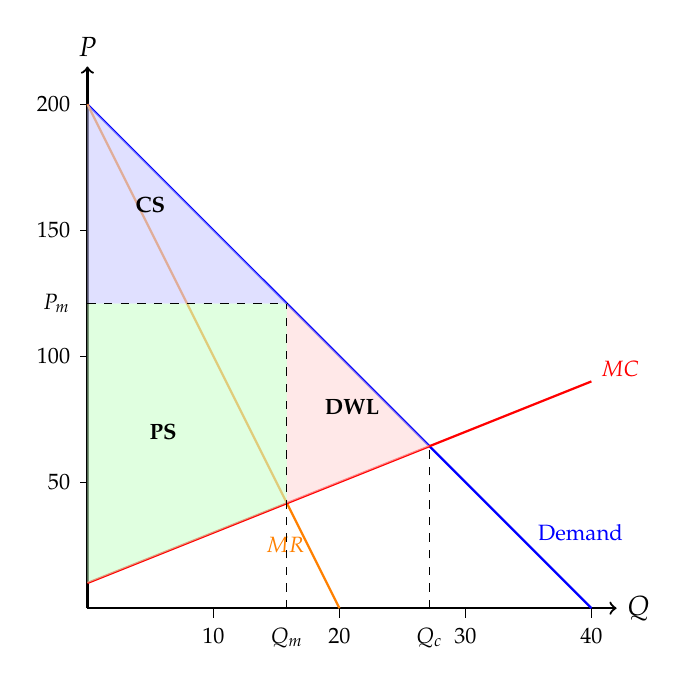
\begin{tikzpicture}[xscale=0.16, yscale=0.032]
    % Axes  (Q from 0..40, P from 0..210)
    \draw[->, thick] (0,0) -- (42,0) node[right] {$Q$};
    \draw[->, thick] (0,0) -- (0,215) node[above] {$P$};
    
    % Tick marks on axes
    \foreach \q in {10,20,30,40} \draw (\q,0) -- (\q,-4) node[below, font=\footnotesize] {$\q$};
    \foreach \p in {50,100,150,200} \draw (0,\p) -- (-0.6,\p) node[left, font=\footnotesize] {$\p$};
    
    % Demand: P = 200 - 5Q  (Q=0,P=200  to  Q=40,P=0)
    \draw[thick, blue] (0,200) -- (40,0);
    \node[blue, font=\footnotesize, anchor=west] at (35,30) {Demand};
    
    % MR: P = 200 - 10Q  (Q=0,P=200  to  Q=20,P=0)
    \draw[thick, orange] (0,200) -- (20,0);
    \node[orange, font=\footnotesize, anchor=east] at (18,25) {$MR$};
    
    % MC: P = 10 + 2Q  (Q=0,P=10  to  Q=40,P=90)
    \draw[thick, red] (0,10) -- (40,90);
    \node[red, font=\footnotesize, anchor=west] at (40,95) {$MC$};
    
    % Monopoly point: Qm=15.83, Pm=120.83, MCm=41.67
    % Competitive point: Qc=27.14, Pc=64.29
    
    % CS Area (triangle above Pm, left of demand)
    \fill[blue!20, opacity=0.6] (0,200) -- (0,120.83) -- (15.83, 120.83) -- cycle;
    
    % PS Area (area between Pm and MC, from 0 to Qm)
    \fill[green!20, opacity=0.6] (0,120.83) -- (15.83, 120.83) -- (15.83, 41.67) -- (0,10) -- cycle;
    
    % DWL Area (triangle between Demand, MC, from Qm to Qc)
    \fill[red!15, opacity=0.6] (15.83, 120.83) -- (27.14, 64.29) -- (15.83, 41.67) -- cycle;
    
    % Dashed lines for Qm, Pm
    \draw[dashed] (15.83, 0) -- (15.83, 120.83);
    \node[font=\footnotesize, below] at (15.83, -4) {$Q_m$};
    \draw[dashed] (0, 120.83) -- (15.83, 120.83);
    \node[font=\footnotesize, left] at (-0.6, 120.83) {$P_m$};
    
    % Dashed line for Qc
    \draw[dashed] (27.14, 0) -- (27.14, 64.29);
    \node[font=\footnotesize, below] at (27.14, -4) {$Q_c$};
    
    % Labels for surplus areas
    \node[font=\footnotesize] at (5, 160) {\textbf{CS}};
    \node[font=\footnotesize] at (6, 70) {\textbf{PS}};
    \node[font=\footnotesize] at (21, 80) {\textbf{DWL}};
\end{tikzpicture}
\end{center}

\section*{6. How are markets defined? List the two dimensions and explain the difference between them. (2 points)}

Markets are formally defined along two primary dimensions:
\begin{enumerate}[leftmargin=*]
    \item \textbf{Product Market Dimension}: Defines the specific bounds of the goods or services being sold based on their degree of substitutability. For instance, whether the market is broadly defined as "all analgesics" or narrowly as "prescription brand-name opioids".
    \item \textbf{Geographic Market Dimension}: Defines the physical or spatial boundaries within which buyers and sellers interact and substitution could realistically occur. For example, a hospital operates in a highly localized, county-level geographic market since patients rarely travel across the country for emergency care, whereas a pharmaceutical manufacturer operates in a global geographic market.
\end{enumerate}

\section*{7. Calculate HHIs... (4 points total)}

\textbf{a) Calculate the HHI for a hospital market with 5 hospitals having shares of 40\%, 25\%, 20\%, 10\%, and 5\%. (1 point)} \\
$HHI = 40^2 + 25^2 + 20^2 + 10^2 + 5^2 = 1600 + 625 + 400 + 100 + 25 = \textbf{2,750}$.

\textbf{b) Calculate the HHI for a market with 250 equally-sized physician practices. (1 point)} \\
Each practice has a market share of $\frac{100\%}{250} = 0.4\%$. \\
$HHI = 250 \times (0.4)^2 = 250 \times 0.16 = \textbf{40}$.

\textbf{c) The DOJ typically considers markets with HHI > 2,500 to be "highly concentrated." Based on your answer to part (a), would this hospital market be considered highly concentrated? What does this suggest about competition in this market? (2 points)} \\
Yes, with an HHI of 2,750 (which strictly exceeds the 2,500 threshold), this hospital market is officially categorized as \textbf{highly concentrated}. This suggests that the market lacks robust, competitive dynamics. A few dominant hospital systems control the vast majority of patients, which strongly implies they wield pronounced market power and could potentially actively dictate higher prices, dictate network terms to insurers, or provide lower structural quality than would exist in a fragmented, competitive environment.

\section*{8. Explain how hospital consolidation affects Market structure, Market power, and Potential impacts on prices. (3 points)}

\begin{itemize}[leftmargin=*]
    \item \textbf{Market Structure (what type of market does it move toward?)}: Consolidation profoundly alters the structure by shifting the local market away from monopolistic competition or a loose oligopoly toward a highly concentrated, tight \textbf{oligopoly} (or even a local \textbf{monopoly}). This results in fewer independent competitors and a surging geographic HHI index.
    \item \textbf{Market Power of Hospitals}: As formerly competing hospitals merge into singular megasystems, their consolidated market share grants them drastically enhanced \textbf{market power}. They transform from price takers (or weak price setters) into dominant entities that form "must-have" networks that health insurance companies absolutely cannot afford to exclude.
    \item \textbf{Potential Impacts on Prices}: Due to the tremendous leverage gained from increased market power, consolidated systems can issue take-it-or-leave-it ultimatums to insurers. Consequently, robust empirical evidence shows that hospital consolidation reliably leads to \textbf{significantly higher prices} for medical procedures and inpatient stays, which are ultimately passed down to consumers through higher insurance premiums.
\end{itemize}

\end{document}
